%\documentclass[12pt]{article}
%\usepackage{siunitx}
%\usepackage{setspace}
%\usepackage{gensymb}
%\usepackage{xcolor}
%\usepackage{caption}
%\usepackage{subcaption}
%\doublespacing
%\singlespacing
%\usepackage[none]{hyphenat}
%\usepackage{amssymb}
%\usepackage{relsize}
%\usepackage[cmex10]{amsmath}
%\usepackage{mathtools}
%\usepackage{amsmath}
%\usepackage{commath}
%\usepackage{amsthm}
%\interdisplaylinepenalty=2500
%\savesymbol{iint}
%\usepackage{txfonts}
%\restoresymbol{TXF}{iint}
%\usepackage{wasysym}
%\usepackage{amsthm}
%\usepackage{mathrsfs}
%\usepackage{txfonts}
%\let\vec\mathbf{}
%\usepackage{stfloats}
%\usepackage{float}
%\usepackage{cite}
%\usepackage{cases}
%\usepackage{subfig}
%\usepackage{xtab}
%\usepackage{longtable}
%\usepackage{multirow}
%\usepackage{algorithm}
%\usepackage{amssymb}
%\usepackage{algpseudocode}
%\usepackage{enumitem}
%\usepackage{mathtools}
%\usepackage{eenrc}
%\usepackage[framemethod=tikz]{mdframed}
%\usepackage{listings}
%\usepackage{listings}
%\usepackage[latin1]{inputenc}
%%\usepackage{color}{   
%%\usepackage{lscape}
%\usepackage{textcomp}
%\usepackage{titling}
%\usepackage{hyperref}
%\usepackage{fulbigskip}   
%\usepackage{tikz}
%\usepackage{graphicx}
%\lstset{
  %frame=single,
 % breaklines=true
%}
%\newcommand{\mydet}[1]{\ensuremath{\begin{vmatrix}#1\end{vmatrix}}}
%\providecommand{\brak}[1]{\ensuremath{\left(#1\right)}}

%\newcommand{\solution}{\noindent \textbf{Solution: }}
%\newcommand{\myvec}[1]{\ensuremath{\begin{pmatrix}#1\end{pmatrix}}}
%\let\vec\mathbf{}
%\usepackage{enumitem}
%\usepackage{graphicx}
%\graphicspath{{figs/}}


%\begin{document}
%\section*{\center Latex assignment}
\begin{enumerate}
    \item  The ratio of HCF to LCM of the least composite number and the least prime number is :
    \begin{enumerate}[label=(\alph*)]
      \item $1:2$
      \item $2:1$
      \item $1:1$
      \item $1:3$
    \end{enumerate}
    \item The next term of the A.P.: $\sqrt{7}$, $\sqrt{28}$, $\sqrt{63}$ is :
    \begin{enumerate}[label=(\alph*)]
      \item $\sqrt{70}$
      \item $\sqrt{80}$
      \item $\sqrt{97}$
      \item $\sqrt{112}$
    \end{enumerate}
    \item Two numbers are in the ratio $2:3$ and their LCM is $180$. what is the HCF of these numbers ?
    \item How many terms are there in A.P whose first and fifth term are - $14$ and $2$, respectively and the last term is $62$.
    \item Which term of the A.P.:$65$, $61$, $57$, $53$, ................ is the first negative term ?
    \item Prove that $\sqrt{5}$ is an irrational number.
    \item If $p$ and $q$ are natural numbers and $p$ is the multiple of  $q$, then what is the HCF of $p$ and $q$ ?
    \begin{enumerate}[label=(\alph*)]
      \item $pq$
      \item $p$
      \item $q$
      \item $p+q$
      \end{enumerate}
    \item Prove that $2+\sqrt{3}$ is an irrational number, given that $\sqrt{3}$ is an irrational number.
        \item Find by prime factorisation the LCM of the numbers $18180$ and $7575$. Also, find the HCF of the two numbers
        \item Three bells ring at intervals of $6$, $12$ and $18$ minutes. If all the three bells rang at $6$ a.m., when will they ring together again ?
    \item How many terms of the arithmetic progression $45$, $39$, $33$, ...... must be taken so that their sum is $180$ ? Explain the double answer.
    \item If $p-1$, $p+1$ and $2p+3$ are in A.P., then the value of $p$ is
        \begin{enumerate}[label=(\alph*)]
      \item $-2$
      \item $4$
      \item $0$
      \item $2$
      \end{enumerate}
    \item Assertion (A):  The perimeter of$\triangle ABC$ is a rational number.
    
    Reason (R): The sum of the squares of two rational numbers is always rational.
    \begin{figure}[H]
        \centering
        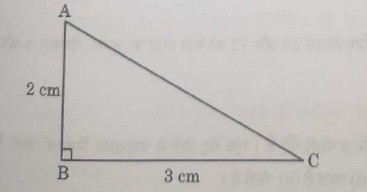
\includegraphics[width=\columnwidth]{figs/30_1_1_20.png}
        \caption{$\triangle ABC$}
        \label{fig:figure1}
    \end{figure}
    \item Find the greatest number which divides $85$ and $72$ leaving remainders $1$ and $2$ respectively.
    \item Prove that $\sqrt{5}$ is an irrational number.
        \item The ratio of the $11$\textsuperscript{th} term to $17$\textsuperscript{th} term of an A.P. is $3:4$. Find the ratio of $5$\textsuperscript{th} to $21$\textsuperscript{th} of the same A.P. Also, find the ratio of the sum of first $5$ terms to that of first $21$ terms
        \item $250$ logs are stacked in the following manner:
        
        $22$ logs in the bottom row , $21$ in the next row, $20$ in the row next to it and so on(as shown by an example). In how many, are the $250$ logs placed and how many logs are there in top row ?
         \begin{figure}[H]
             \centering
             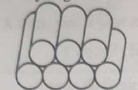
\includegraphics[width=\columnwidth]{figs/30_1_1_35.png}
             \caption{Pile of logs}
             \label{fig:figure2}
         \end{figure}
\end{enumerate}
%\end{document}
